%\documentclass[11pt]{article}
\documentclass[11pt,onecolumn]{scrartcl}
%\documentclass[11pt,onecolumn,fleqn]{scrartcl}
\usepackage[utf8]{inputenc}
\usepackage{amsmath,amssymb,amsfonts,mathrsfs,amsthm}
\usepackage[top=2cm,bottom=3cm,left=2.5cm,right=2cm]{geometry}
\usepackage{amssymb}
\usepackage{listings}
\usepackage{array}
\usepackage{mathtools}
\usepackage{dsfont}
\usepackage{graphicx}
\usepackage{pdfpages}
%\usepackage[textsize=footnotesize,color=green]{todonotes}
\usepackage{algorithm, algorithmic}
\usepackage{tikz}
\usepackage{subfigure}
%\usetikzlibrary{%
%    decorations.pathreplacing,%
%    decorations.pathmorphing%
%}
\usepackage[normalem]{ulem}

\newcommand{\bs}[1]{\boldsymbol{#1}}
\DeclareMathOperator{\diag}{diag}

\newcommand{\equaldef}{\stackrel{\mathrm{def}}{=}}

\newcommand{\tablab}[1]{\label{tab:#1}}
\newcommand{\tabref}[1]{Table~\ref{tab:#1}}

\newcommand{\theolab}[1]{\label{theo:#1}}
\newcommand{\theoref}[1]{\ref{theo:#1}}
\newcommand{\eqnlab}[1]{\label{eq:#1}}
\newcommand{\eqnref}[1]{\eqref{eq:#1}}
\newcommand{\seclab}[1]{\label{sec:#1}}
\newcommand{\secref}[1]{\ref{sec:#1}}
\newcommand{\lemlab}[1]{\label{lem:#1}}
\newcommand{\lemref}[1]{\ref{lem:#1}}

\newcommand{\mb}[1]{\mathbf{#1}}
\newcommand{\mc}[1]{\mathcal{#1}}
\newcommand{\nor}[1]{\left\| #1 \right\|}
\newcommand{\snor}[1]{\left| #1 \right|}
\newcommand{\LRp}[1]{\left( #1 \right)}
\newcommand{\LRs}[1]{\left[ #1 \right]}
\newcommand{\LRa}[1]{\left< #1 \right>}
\newcommand{\LRc}[1]{\left\{ #1 \right\}}
\newcommand{\tanbui}[2]{\textcolor{blue}{\sout{#1}} \textcolor{red}{#2}}
\newcommand{\Grad} {\ensuremath{\nabla}}
\newcommand{\Div} {\ensuremath{\nabla\cdot}}

\newcommand{\vect}[1]{\ensuremath\boldsymbol{#1}}
\newcommand{\tensor}[1]{\underline{\vect{#1}}}
\newcommand{\del}{\Delta}
\newcommand{\grad}{\nabla}
\newcommand{\curl}{\grad \times}
\renewcommand{\div}{\grad \cdot}
\newcommand{\ip}[1]{\left\langle #1 \right\rangle}
\newcommand{\eip}[1]{a\left( #1 \right)}
\newcommand{\pd}[2]{\frac{\partial#1}{\partial#2}}
\newcommand{\pdd}[2]{\frac{\partial^2#1}{\partial#2^2}}

\newcommand{\circone}{\ding{192}}
\newcommand{\circtwo}{\ding{193}}
\newcommand{\circthree}{\ding{194}}
\newcommand{\circfour}{\ding{195}}
\newcommand{\circfive}{\ding{196}}

\def\arr#1#2#3#4{\left[
\begin{array}{cc}
#1 & #2\\
#3 & #4\\
\end{array}
\right]}
\def\vecttwo#1#2{\left[
\begin{array}{c}
#1\\
#2\\
\end{array}
\right]}
\def\vectthree#1#2#3{\left[
\begin{array}{c}
#1\\
#2\\
#3\\
\end{array}
\right]}
\def\vectfour#1#2#3#4{\left[
\begin{array}{c}
#1\\
#2\\
#3\\
#4\\
\end{array}
\right]}

\newtheorem{proposition}{Proposition}
\newtheorem{corollary}{Corollary}
\newtheorem{theorem}{Theorem}
\newtheorem{lemma}{Lemma}

\newcommand{\G} {\Gamma}
\newcommand{\Gin} {\Gamma_{in}}
\newcommand{\Gout} {\Gamma_{out}}

\begin{document}

\section{Introduction}

\subsection{Introduction to DPG}
The idea of optimal test functions was introduced by Demkowicz and Gopalakrishnan in \cite{DPG2}.  Conceptually, these optimal test functions are the result of a minimum residual method applied to the operator form of a variational equation.  Given Hilbert spaces $U$ and $V$ and a the variational problem $b(u,v) = l(v)$, $\forall u\in U, v\in V$, we can identify $B:U\rightarrow V'$ and $l \in V'$ 
\[
\left.\begin{array}{c}
b(u_h,v) = \langle Bu_h,v\rangle  \\
l(v) = \langle l,v\rangle
\end{array}\right\}
\Longleftrightarrow Bu_h = l
\]
We seek the minimization of the residual in the dual norm
\[
\min_{u_h\in U_h} J(u_h) = \frac{1}{2}\|Bu_h-l\|_{V'}^2 = \frac{1}{2} \sup_{v\in V} \| b(u_h,v)-l(v)\|_{V}^2
\]
Recall $R_V$, the Riesz operator $\langle R_V v,\delta v\rangle = (v, \delta v)_V$ identifying elements of Hilbert space with elements of the dual.  As $R_V$ and its inverse are isometries, $\|f\|_{V'} = \|R_V^{-1} f\|_V$, and 
\[
\min_{u_h\in U_h} J(u_h) = \frac{1}{2}\|Bu_h-l\|_{V'}^2 =  \frac{1}{2}\|R_V^{-1}(Bu_h-l)\|_V^2
\]
First order optimality conditions require the Gateux derivative to be zero in all directions $u_h \in U_h$.  
\begin{align*}
\left(R_V^{-1}(Bu_h-l),R_V^{-1}B\delta u_h\right)_V &= 0, \quad \forall \delta u_h \in U_h \\
\rightarrow \langle Bu_h-l, v_h\rangle &= 0, \quad v_h = R_V^{-1}B\delta u_h
\end{align*}
which returns a standard variational equation $b(u_h,v_h) - l(v_h) = 0$, for the specific choice of test functions $v_h = R_V^{-1}B\delta u_h$.  We identify the \textit{trial-to-test} operator $T = R_V^{-1}B$, which maps a trial function $u_h$ to its corresponding \textit{optimal} test function $v_h = Tu_h$.  These test functions can be solved for by solving the auxiliary variational problem
\[
\left(v_h,\delta v\right)_V = b(u_h,v)
\]

Finally, while the above variational problem is a global operation for standard continuous test spaces, the use of discontinuous test spaces reduces it to an element-local problem.  In practice, this variational problem can rarely be solved exactly and it is solved approximately using the standard Bubnov-Galerkin method and an ``enriched" subspace of $V$. We assume the corresponding error in approximation of the optimal test functions is negligible for the scope of this paper.  Further work concerning the effect of approximation error in the computation of optimal test functions can be found in \cite{practicalDPG}.

Under the standard conditions for well-posedness of the continuous variational problem, the discrete DPG method delivers the best approximation error in the ``energy norm" $\|u\|_E = \sup \frac{b(u,v)}{\|v\|_V}$.  Additionally, the actual energy error $\|u-u_h\|_E$ is computable through $\|e_h\|_V$, where
\[
\left(e_h,\delta v\right)_V = b(u-u_h,v) = b(u_h,v)-l(v)
\]
This is simply a consequence of the least-squares nature of DPG; the energy error is simply the measure of the residual in the proper norm.  

\subsection{Variational form}

The DPG (discontinuous Petrov-Galerkin) method is the combination of the concept of computable optimal test functions with the so-called ``ultra-weak formulation", where every equation is relaxed.  Moreover, to maintain conformity while seeking an $L^2$ setting on interior ``field" variables, boundary terms are identified as additional new unknowns.  The result is a hybrid DG method with locally supported optimal test functions.  For a given operator equation $Au = f$, the ultra-weak formulation is 
\[
b\left(\left(\widehat{u},u\right),v\right) - l(v) = \langle \widehat{u}, v \rangle - (u,A^*v) - (f,v)
\]

\section{Choice of test norm}

Up to now, we've neglected discussion of the proper choice of inner product/norm on the space $V$.  This choice is important, as the choice of norm on $V$ determines the 

Under the assumption of injectivity of the adjoint of our variational operator $B$, we can define the optimal test norm 
\[
\|v\|_{\rm opt} = \sup_{u\in U}\frac{b(u,v)}{\|u\|_U}
\]
If the solution is in $U$, then choosing $\|v\|=\|v\|_{\rm opt}$ implies 
\[
\|u\|_E = \sup_{v\in V}\frac{b(u,v)}{\|v\|_V} = \sup_{v\in V}\sup_{w\in V}\frac{b(u,v)}{b(w,v)}\|w\|_U =\sup_{w\in V}\frac{b(u,v^*)}{b(w,v^*)}\|w\|_U = \|u\|_U
\]
FIX ABOVE 

This norm is non-localizable, however - even with discontinuous test functions, solving for optimal test functions under this optimal norm will result in global problems as well, due to the coupling given by the boundary terms in our bilinear form.  The ``quasi-optimal" test norm is created by removing such boundary terms and replacing them with scaled $L^2$ norms of the field variables.  

\subsection{Singular perturbation problems and robustness}

Standard Bubnov-Galerkin methods tend to perform poorly for the class of partial-differential equations known as singularly perturbed problems, where a given parameter $\epsilon$ may approach either $0$ or $\infty$ in the context of physical problems.  This poor performance is captured by the error bound
\[
\|u-u_h\|_E \leq C(\epsilon) \inf_{w_h}\|u-w_h\|_U
\]
The growth of $C$ with $\epsilon$ is referred to as a loss of robustness, where the bound on the error in the finite element solution by the best approximation error.  Intuitively, as our singular perturbation parameter changes, our finite element error is bounded more and more loosely to the best approximation error, allowing for degradation of the solution   

A well-known example is the growth of spurious oscillations in the finite element solution of the 1D convection-diffusion problem $ u'-\epsilon u'' = f$ (with Dirichlet boundary conditions) as $\epsilon\rightarrow 0$.  Another class of examples are wave propagation problems, in which the singular perturbation parameter is the wavenumber, $k\rightarrow \infty$.  The lack of robustness in this case manifests as ``pollution" error, a phenomenon where the finite element solution degrades over many wavelengths (commonly manifesting as a phase error between the FE solution and the exact solution).  The DPG method is currently being analyzed for both acoustic and elastic waves in context of the Helmholtz equation \cite{DPG4} and equations of linear elasticity.  Numerically, DPG appears to yield a ``pollution-free" method for these problems under a specific regularization of the ``quasi-optimal" test norm.  

\section{Model problem and robustness using DPG}

We consider the model convection-diffusion problem on domain $\Omega$ with boundary $\Gamma$
\begin{align*}
\div (\beta u - \sigma) &= f \\
\frac{1}{\epsilon}\sigma - \grad u &= 0
\end{align*}
with the corresponding variational form 
\[
b\left(\left(u,\sigma, \widehat{u}, \widehat{\sigma}_n\right), \left(\tau, v\right)\right) = \left(u,\div \tau - \beta \cdot \grad v\right) + \left(\sigma, \epsilon^{-1} \tau + \grad v\right) - \langle \left[\tau_n\right], \widehat{u} \rangle + \langle \widehat{f}_n, \left[v\right] \rangle
\]
where the above inner products are taken element-wise over the finite element mesh $\Omega_h$, and the duality pairings are taken on $\Gamma_h$, the mesh ``skeleton", or union of edges of elements $K$ in $\Omega_h$.  Define the interior skeleton $\Gamma_h^0 = \Gamma_h \setminus \Gamma$.  The functional setting is now well understood as well (see \cite{analysisDPG} for details) - $u,\sigma \in L^2(\Omega)$, $v \in H^1(\Omega_h)$, $\tau \in H({\rm div},\Omega_h)$, where $H^1(\Omega_h)$ and $H({\rm div},\Omega_h)$ are element-wise ``broken" Sobolev spaces.  By duality, $\widehat{u}$ lives in the trace space of $H^1(\Omega_h)$, while $\widehat{f}_n$ comes from the normal trace space of $H({\rm div},\Omega_h)$.  

To analyze the robustness of DPG, we note that 
\[
b\left(\left(u,\sigma, \widehat{u}, \widehat{\sigma}_n\right), \left(\tau, v\right)\right) = \| u \|^2_{L^2}
\]
for the specific continuous test functions $\tau$ and $v$ satisfying
\begin{align*}
\div \tau - \beta \cdot \grad v &= g \\
\frac{1}{\epsilon}\tau + \grad v &= f
\end{align*}
with $g=u$ and $f=0$, and with boundary conditions such that the boundary terms in the bilinear form vanish.  Then, for the above choice of $\left(\tau, v\right)$, 
\begin{align*}
\|u\|_{L^2}^2 &= b\left(\left(u,\sigma, \widehat{u}, \widehat{\sigma}_n\right), \left(\tau, v\right)\right) = \frac{b\left(\left(u,\sigma, \widehat{u}, \widehat{\sigma}_n\right), \left(\tau, v\right)\right)}{\|\left(\tau, v\right)\|_V}\|\left(\tau, v\right)\|_V \leq \|u\|_E \|\left(\tau, v\right)\|_V
\end{align*}
We will use the notation $\lesssim$ to denote an $\epsilon$-independent bound.  If we can show $\|\left(\tau, v\right)\|_V \lesssim \| u \|_{L^2}$ for any choice of $u \in L^2$, then dividing through by $\|u\|_{L^2}$ gives
\[
\|u\|_{L^2} \lesssim \|u\|_E
\]
which results in in robust control of the $L^2$ error by the error in the energy norm, in which DPG is optimal.  The study of robustness for the DPG method has now been reduced to proving stability estimates for the adjoint problem.  

For convection-diffusion, the quasi-optimal norm is 
\[
\|\left(\tau, v\right)\|_V^2 = \| \div \tau - \beta \cdot \grad v \|_{L^2}^2 + \| \epsilon^{-1} \tau + \grad v \|_{L^2}^2 + C_1\|v\|_{L^2} + C_2\|\tau\|_{L^2}
\]
for some choice of constants $C_1$ and $C_2$.  We note that the optimal test norm will automatically guarantee the robust bound $\|\left(\tau, v\right)\|_V \leq \|u\|_{L^2}$.  However, use of this norm for the convection-diffusion problem is difficult - the variational problem for optimal test functions using the quasi-optimal test norm is equivalent to a reaction-diffusion system \cite{DBLP:journals/procedia/NiemiCC11}.  Transforming the problem to the reference element reveals that will induce strong boundary layers of width $\epsilon/h^2$ (in comparison, in wave propagation problems, the mesh size tends to be on the order of the wavelength/singular perturbation parameter, resulting in smooth optimal test functions that are much easier to approximate over the reference element).  As the relevant range of $\epsilon$ for physical problems is $1e-7$, solving on partially under-resolved meshes is unavoidable.  Resolving such boundary layers for an underresolved mesh has been investigated numerically using specially designed subgrid meshes by Niemi, Collier, and Calo in \cite{DBLP:journals/procedia/NiemiCC11}.  We approach this from a different perspective, looking instead for robust test norms which do not induce boundary layers in the approximation of optimal test functions.  

\subsection{Boundary conditions}

We split the boundary $\Gamma$ into three portions
\begin{align*}
\Gamma_{-} &\coloneqq \{x\in \Gamma; \beta_n(x) < 0\} \quad {\rm (inflow)}\\
\Gamma_{+} &\coloneqq \{x\in \Gamma; \beta_n(x) > 0\} \quad {\rm (outflow)}\\
\Gamma_{0} &\coloneqq \{x\in \Gamma; \beta_n(x) = 0\}\\
\end{align*}
Demkowicz and Heuer proved in \cite{DPGrobustness} that for Dirichlet boundary conditions everywhere on $\Gamma$, robustness as $\epsilon \rightarrow 0$ is achieved by the test norm
\[
\|\left(\tau, v\right)\|_{V,w}^2 = \|v\| + \epsilon \|\grad v\| + \|\beta \cdot \grad v\|_{w+\epsilon} + \| \div \tau\|_{w+\epsilon} + \frac{1}{\epsilon}\|\tau\|_{w+\epsilon}
\]
where $\|\cdot \|_{w+\epsilon}$ is a weighted $L^2$ norm, where the weight $w \in (0,1)$ is required to vanish on $\Gamma_-$.  The need for the weight is intuitively explained by the induced adjoint problem.  The bilinear form for the Dirichlet case is
\[
b\left(\left(u,\sigma, \widehat{u}, \widehat{\sigma}_n\right), \left(\tau, v\right)\right) = \left(u,\div \tau - \beta \cdot \grad v\right) + \left(\sigma, \epsilon^{-1} \tau + \grad v\right) + \langle \widehat{f}_n, \left[v\right] \rangle
\]
Choosing a continuous conforming test function $v$ removes the contribution of the term $\langle \widehat{f}_n, \left[v\right] \rangle$ on the mesh skeleton; however, it is necessary to assume in addition $v=0$ on $\Gamma$ to have 
$$b\left(\left(u,\sigma, \widehat{u}, \widehat{\sigma}_n\right), \left(\tau, v\right)\right) = \|u\|_{L^2}^2.$$  Intuitively, the adjoint problem is similar to the primal problem with the direction of inflow reversed, such that the inflow becomes the outflow, and outflow inflow.  The need for the weight arises due to the presence of the Dirichlet boundary condition on $v$ near the inflow; this induces strong boundary layers at the inflow such that $\grad v \approx O(\epsilon^{-1})$. It may be of interest to note that, for sufficiently small $\epsilon$, these issues manifest themselves in numerical experiments as additional refinements near the inflow.

We improve upon the result of Demkowicz and Heuer by adopting a new inflow boundary condition, given by Hesthaven et al in \cite{Hesthaven96astable}, where we set
\[
\beta_n u - \sigma_n = f_n = u_0
\]
on $\Gamma_-$, and continue with the wall boundary condition $u=0$ on $\Gamma_+$.  For our model problem, as for most problems of interest in CFD, we expect $\grad u$ to be small near the inflow, and that the solution using $u=u_0$ and $\beta_n u - \sigma_n = f_n = u_0$ should converge to each other for sufficiently small $\epsilon$.  

Under the new inflow conditions, the induced bilinear form is now
\[
b\left(\left(u,\sigma, \widehat{u}, \widehat{\sigma}_n\right), \left(\tau, v\right)\right) = \left(u,\div \tau - \beta \cdot \grad v\right) + \left(\sigma, \epsilon^{-1} \tau + \grad v\right) - \langle \left[\tau_n\right], \widehat{u} \rangle_{\Gamma_-} + \langle \widehat{f}_n, \left[v\right] \rangle_{\Gamma_+}
\]
The corresponding adjoint problem now has boundary conditions
\begin{align}
\tau_n &= 0, \quad x\in \Gamma_-\cup \Gamma_0 \label{eq:adj_bc1}\\
v &= 0, \quad x\in \Gamma_+ \label{eq:adj_bc2}
\end{align}
and it can be shown that DPG is robust using an unweighted version of the test norm in \cite{DPGrobustness}
\[
\|\left(\tau, v\right)\|_{V}^2 = \|v\| + \epsilon \|\grad v\| + \|\beta \cdot \grad v\| + \| \div \tau\| + \frac{1}{\epsilon}\|\tau\|
\]

\subsection{Stability of the adjoint problem (bound from below)}

We reduce the adjoint problem to the scalar second order equation
\begin{equation}
- \epsilon \Delta v - \beta \cdot \grad v = g - \epsilon \div f \label{adjoint}
\end{equation}
with boundary conditions
\begin{align*}
\tau_n = - \epsilon \grad v \cdot n &=f\cdot n, \quad x\in \Gamma_-\\
v &= 0, \quad x\in \Gamma_+ 
\end{align*}
and treat the cases $f=0$, $g=0$ separately.  The above boundary conditions reduce down to \eqref{eq:adj_bc1} and \eqref{eq:adj_bc2} when requesting $L^2$ robustness in $u$ ($f=0$); these more general boundary conditions are necessary for bounds involving $f \neq 0$.

Additionally, the $\div$ operator is understood now in the weak sense, as the dual operator of $-\grad : H_0^1(\Omega) \rightarrow L^2(\Omega)$, such that $\div f \in \left(H_0^1(\Omega)\right)'$.  $f\cdot n$ is understood as a limit; smooth functions are dense in $H^1(\Omega)$, and we define $f\cdot n$ as the limit of $f_i\cdot n$, where $f_i \in C^\infty(\Omega)$, $f_i \rightarrow f$.

For this analysis, it will be necessary to assume conditions on $\beta$.  For each proof, we require $\beta \in C^2(\bar{\Omega})$ and $\beta, \div \beta = O(1)$.  Additionally, we will assume one or both of the following assumptions
\begin{align}
&\curl \beta = 0, \quad 0<C \leq \left | \beta\right |^2 + \frac{1}{2}\div \beta, \quad C = O(1) \label{a_req}\\
&\grad \beta + \grad \beta ^T - \div \beta I = O(1) \label{b_req}
\end{align}
The second lemma concerns the robust control of $u$ by the energy error; the first and third concern the robust control of field variable $\sigma$ and flux/trace variables, respectively.  

\begin{lemma} 
\label{lemma_1}
Assuming \eqref{a_req} and \eqref{adjoint} hold, for sufficiently small $\epsilon$, 
\[
\epsilon \|\grad v\|^2 + \|v\|^2 \lesssim \|g\| + \epsilon \| f\|
\]
\end{lemma}

\begin{proof}
Since $\curl \beta=0$, and $\Omega$ is simply connected, there exists a scalar potential $\psi$, $\grad \psi = \beta$ such that $e^\psi = O(1)$.  Take the transformed function $w = e^\psi v$; following (2.26) in \cite{DPGrobustness}, we substitute $w$ into the the left hand side of equation \eqref{adjoint}, arriving at the relation  
\[
-\epsilon \Delta w - (1-2\epsilon) \beta \cdot \grad w + \left((1-\epsilon)|\beta|^2 + \epsilon \div \beta\right) w = e^\psi (g-\epsilon \div f)
\]
Multiplying by $w$ and integrating over $\Omega$ gives
\[
-\epsilon \int_\Omega \Delta ww - (1-2\epsilon) \int_\Omega\beta \cdot \grad w w + \int_\Omega\left((1-\epsilon)|\beta|^2 + \epsilon \div \beta\right) w^2 = \int_\Omega e^\psi (g-\epsilon \div f) w
\]
Integrating by parts gives
\[
-\epsilon \int_\Omega \Delta ww - (1-2\epsilon) \int_\Omega\beta \cdot \grad w w = \epsilon \left( \int_\Omega |\grad w|^2- \int_{\Gamma} w \grad w \cdot n  \right) + \frac{(1-2\epsilon) }{2} \left(\int_\Omega \div \beta w^2 - \int_\Gamma\beta_n w^2 \right)
\]
Noting that $w=0$ on $\Gamma_+$ reduces the boundary integrals over $\Gamma$ to just the inflow $\Gamma_-$.  Furthermore, we have the relation $\grad w = e^\psi(\grad v + \beta v)$.  Applying the above and boundary conditions on $\Gamma_-$, the first boundary integral becomes
\[
\int_{\Gamma_-} w \grad w \cdot n = \int_{\Gamma_-} we^\psi(\grad v + \beta v)\cdot n =  \int_{\Gamma_-} we^\psi(f\cdot n + \beta_n v)
\]
Noting $\int_{\Gamma_-}\beta_n w^2 \leq 0$ through $\beta_n<0$ on the inflow gives
\[
\epsilon \int_\Omega |\grad w|^2 + \int_\Omega \left((1-\epsilon)|\beta|^2 + \frac{1}{2} \div \beta \right) w^2 - \epsilon \int_{\Gamma_-} we^\psi f\cdot n \leq \int_\Omega e^\psi (g-\epsilon \div f) w
\]
assuming $\epsilon$ is sufficiently small.  Our assumptions on $\beta$ allow us to bound $\left((1-\epsilon)|\beta|^2 + \frac{1}{2} \div \beta \right) \lesssim 1$ and $e^\psi \lesssim 1$. We can then bound the left hand side from below by
\[
\epsilon \|\grad w\|^2 + \|w\|^2 - \epsilon \int_{\Gamma_-} we^\psi f\cdot n  \lesssim \epsilon \int_\Omega |\grad w|^2 + \int_\Omega \left((1-\epsilon)|\beta|^2 + \frac{1}{2} \div \beta \right) w^2 - \epsilon \int_{\Gamma_-} we^\psi f\cdot n 
\]
Interpreting $\div f$ as a functional, the right hand gives
\begin{align*}
\int_\Omega e^\psi (g-\epsilon \div f) w &= \int_\Omega e^\psi g + \int_\Omega \epsilon f \cdot \grad (e^\psi w) - \int_\Gamma \epsilon f\cdot n e^\psi w\\
\end{align*}
The boundary integral on $\Gamma$ reduces to $\Gamma_-$, which is then nullified by the same term on the left hand side, leaving us with 
\[
\epsilon \|\grad w\|^2 + \|w\|^2 \lesssim \int_\Omega e^\psi g + \int_\Omega \epsilon f \cdot \grad (e^\psi w) = \int_\Omega e^\psi g + \int_\Omega \epsilon f \cdot (\beta w + \grad w)
\]
From here, the proof is identical to \cite{DPGrobustness}; an application of Peter-Paul Young's inequality to the right hand side and bounds on $\|v\|, \|\grad v\|$ by $\|w\|,\|\grad w\|$ complete the estimate.  
%ISSUE: REMOVE BOUNDARY TERM
\end{proof}

\begin{lemma} 
\label{lemma_2}
Assume $v$ satisfies $\eqref{adjoint}$ and $\beta$ satisfies \eqref{a_req} and \eqref{b_req}.  If $\div f = 0$ and $\epsilon$ is sufficiently small, 
\[
\|\beta \cdot \grad v \| \lesssim \| f\|
\]
\end{lemma}

\begin{proof}
Define $v_\beta = \beta\cdot \grad v$.  Multiplying by $v_\beta$ and integrating over $\Omega$ gives
\[
\|v_\beta\|^2 = -\int_\Omega g v_\beta - \epsilon \int_\Omega \Delta v v_\beta
\]
Note that 
\[
-\int_{\Omega} \beta\cdot \grad v \del v = -\int_{\Omega} \beta\cdot \grad v \div \grad v
\]
Integrating this by parts, we get
\[
-\int_{\Omega} \beta\cdot \grad v \div \grad v = \int_{\Omega}\grad (\beta\cdot \grad v) \cdot \grad v  - \int_{\Gamma}n\cdot \grad v \beta\cdot\grad v
\]
Note that 
\[
\grad (\beta \cdot \grad v) = \grad \beta \cdot \grad v + \beta \cdot \grad \grad v
\]
where $\grad \beta$ and $\grad \grad v$ are understood to be tensors. Then, 
\[
\int_{\Omega}\grad (\beta\cdot \grad v) \cdot \grad v = \int_{\Omega}(\grad \beta\cdot \grad v) \cdot \grad v + \int_{\Omega}\beta\cdot \grad\grad v \cdot \grad v 
\]
Noting that $\grad v \cdot \grad \grad v = \grad\frac{1}{2}\left(\grad v\cdot \grad v\right)$, if we integrate by parts again, we get
%\[
%\int_{\Omega}\beta\cdot \grad\grad v \cdot \grad v = \frac{1}{2}\int_{\Omega}\beta\cdot \grad(\grad v \cdot \grad v ) = \frac{1}{2}\int_{\Gamma}\beta_n (\grad v \cdot \grad v ) - \frac{1}{2}\int_{\Omega}\div \beta (\grad v \cdot \grad v )
%\]
%Then, we can combine these terms to get
\begin{align*}
-\int_{\Omega}  \del vv_\beta &= - \int_{\Gamma}n\cdot \grad v \beta\cdot\grad v + \frac{1}{2}\int_{\Gamma}\beta_n (\grad v \cdot \grad v ) - \frac{1}{2}\int_{\Omega}\div \beta (\grad v \cdot \grad v ) + \int_{\Omega}(\grad \beta\cdot \grad v) \cdot \grad v\\
&= - \int_{\Gamma}n\cdot \grad v \beta\cdot\grad v + \frac{1}{2}\int_{\Gamma}\beta_n (\grad v \cdot \grad v ) + \int_{\Omega} \grad v \left(\grad \beta - \frac{1}{2}\div \beta I\right)\grad v
\end{align*}
Finally, substituting this into our adjoint equation multiplied by $v_\beta$, we get
\[
\| v_\beta\|^2 = -\int_{\Omega}g\beta\cdot \grad v +  \epsilon\int_{\Gamma}  \left( -n\cdot \grad v \beta + \frac{1}{2}\beta_n \grad v \right) \cdot \grad v + \epsilon\int_{\Omega} \grad v \left(\grad \beta - \frac{1}{2}\div \beta I\right)\grad v
\]
%The first term on the RHS can be controlled using Young's inequality. 
The last term can be bounded by our assumption on $\|\grad \beta - \frac{1}{2}\div \beta I\|^2 \leq C$.
\[
\epsilon \int_{\Omega} \grad v \left(\grad \beta - \frac{1}{2}\div \beta I\right)\grad v \leq C\frac{\epsilon}{2} \|\grad v\|^2
\]
For the boundary terms, on $\Gamma_-$, $\grad v\cdot n = 0$, reducing the above to $\beta_n|\grad v|^2 \leq 0$.  On $\Gamma_+$, $v=0$ implies $\grad v \cdot \tau = 0$, where $\tau$ is a tangential direction.  An orthogonal decomposition yields $\grad v = (\grad v \cdot n) n$, reducing the above to 
\[
 \epsilon\int_{\Gamma}  -\frac{1}{2}|\beta_n| (\grad v \cdot n)^2 \leq 0
\]
leaving us with the estimate
\[
\|v_\beta\|^2 \leq  -\int_{\Omega}g\beta\cdot \grad v + C\frac{\epsilon}{2} \|\grad v\|^2
\]
Since $C=O(1)$, an application of Young's inequality and Lemma 1 complete the estimate.
\end{proof}

\begin{lemma}
\label{lemma_3}
Let $\beta$ satisfy \eqref{a_req} and $\div \beta = 0$, and $f=g=0$.  Then, there holds
\[
\|\grad v\| = \frac{1}{\epsilon}\|\tau\| \lesssim \frac{1}{\epsilon} \| [\tau\cdot n]\|_{\Gamma_h \setminus \Gamma_+} + \frac{1}{\sqrt{\epsilon}} \| [v]\|_{\Gamma_h^0 \cup \Gamma_+}
\]
\end{lemma}
\begin{proof}
We follow \cite{analysisDPG} and \cite{DPGrobustness} in decomposing $\tau$ into $z\in H({\rm curl},\Omega)$ and $\psi\in H^1(\Omega)$ such that
\[
\tau = \left(\epsilon \grad \psi - \beta \psi\right) + \curl z
\]
Specifically, $\psi$ is chosen as the solution to 
\begin{align*}
-\epsilon \grad \psi + \div \left(\beta \psi\right) &= -\div \tau \\
\epsilon \grad \psi \cdot n - \beta_n \psi - \tau\cdot n &= 0, \quad x\in \Gamma_-\\
\psi &= 0, \quad x\in \Gamma_+ 
\end{align*}
Since $\div \beta = 0$, we satisfy \eqref{a_req}, and can use Lemma 1 (with $f = \frac{1}{\epsilon}\tau$) to bound
\[
\epsilon \|\grad \psi\|^2 + \|\psi \|^2 = \frac{1}{\epsilon}\|\tau\|^2
\]
By the above bound and triangle inequality, 
\[
\|\curl z \| \leq \epsilon \|\grad \psi\| + \|\beta \psi\| + \|\tau\| \lesssim \frac{1}{\sqrt{\epsilon}}\|\tau\|
\]
On the other hand, using the decomposition and boundary conditions directly, we have
\begin{align*}
\|\tau\|^2 &= (\tau, \epsilon \grad \psi - \beta \psi + \curl z) = (\tau, \epsilon \grad \psi) - (\tau,\beta \psi) + (\tau,\curl z)  \\
&=(\tau, \epsilon \grad \psi) + \epsilon(\grad v,\beta \psi) - \epsilon(\grad v,\curl z)  \\
&=\epsilon \langle [\tau \cdot n],\psi \rangle - \epsilon  \langle n\cdot \curl z, [v]\rangle = \epsilon \langle [\tau \cdot n],\psi \rangle_{\Gamma_h \setminus \Gamma_+} - \epsilon  \langle n\cdot \curl z, [v]\rangle_{\Gamma_h \cup \Gamma_+}\\
&\lesssim \epsilon \|[\tau \cdot n]\|_{\Gamma_h \setminus \Gamma_+} \|\psi\| + \epsilon \| [v]\|_{\Gamma_h \cup \Gamma_+}\| n\cdot \curl z \| 
\end{align*}
by the boundary norms, which are defined by duality
\begin{align*}
\|[\tau\cdot n]\|_{\Gamma_h} &\coloneqq \sup_{w\in H^1} \frac{\langle [\tau \cdot n], w\rangle}{\|w\|_{H^1(\Omega)}}\\
\|[v]\|_{\Gamma_h} &\coloneqq \sup_{\eta\in H({\rm div})} \frac{\langle v, \eta\cdot n\rangle}{\|\eta\|_{H({\rm div},\Omega)}}
\end{align*}
Applying the above estimates for $\|\psi\|$ and $\|n\cdot \curl z\|$ and noting that $\|\grad v\| = \frac{1}{\epsilon}\|\tau\|$ completes the proof.
\end{proof}
\subsection{Energy norm equivalence (bound from above)}

TODO: FINISH THIS.

\section{Numerical experiments}

In our numerical experiments, we will be interested in the use of the unweighted test norm 
\[
\|\left(\tau, v\right)\|_{V}^2 = \|v\| + \epsilon \|\grad v\| + \|\beta \cdot \grad v\| + \| \div \tau\| + \frac{1}{\epsilon}\|\tau\|
\]
However, the presence of both $\|v\|$ and $\epsilon\|\grad v\|$ terms, and similarly $\|\div \tau\|$ and $\frac{1}{\epsilon}\|\tau\|$ terms, induces boundary layers in the optimal test functions, though only in the crosswind direction.  To avoid this effect, we follow \cite{DPGrobustness} in scaling the $L^2$ contributions of $v$ and $\tau$ such that, when transformed to the reference element, both $v$ and $\grad v$ terms are $O(1)$.  In this paper, we consider only isotropic refinements on quadrilateral elements, such that $h_1 = h_2 = h$, and $|K| = h^2$.
\[
\|\left(\tau, v\right)\|_{V}^2 = \min\left\{\frac{\epsilon}{|K|},1\right\}\|v\| + \epsilon \|\grad v\| + \|\beta \cdot \grad v\| + \| \div \tau\| + \min\left\{\frac{1}{\epsilon},\frac{1}{|K|}\right\}\|\tau\|
\]
This modified test norm avoids boundary layers, but for adaptive meshes, provides additional stability in areas of heavy refinement.  Intuitively, this is justifiable by the fact that best approximation error is typically largest near boundary layers, where refinements tend to aggregate.  Additionally, test norms that differ from element to element fit cleanly into the DPG framework - as the best approximation error tends to be negligible in areas where the solution is smooth, the finite element error will be small in those areas, even with slightly suboptimal robustness.

\subsection{Erickson model problem}

For the choice of $\Omega = [0,1]^2$ and $\beta = (1,0)^T$, the convection diffusion equation reduces to
\[
\pd{u}{x} - \epsilon \left(\pdd{u}{x}+ \pdd{u}{y}\right) = f
\]
which, for $f=0$, has an exact solution by separation of variables, allowing us to analyze convergence of DPG for a wide range of $\epsilon$.  For boundary conditions, we impose $u=0$ on $\Gamma_+$ and $\beta_n u - \sigma_n$ on $\Gamma_-$, which reduces to
\begin{align*}
u-\sigma_x &= u_0-\sigma_{x,0}, \quad x=0\\
\sigma_y &=  0, \quad y=0,1\\
\end{align*}
In this case, our exact solution is the series
\[
u(x,y) = C_0 + \sum_{n=1}^\infty C_n \frac{\exp(r_2(x-1)-\exp(r_1(x-1)))}{r_1\exp(-r2) - r_2\exp(-r1)}\cos(n\pi y)
\]
where
\begin{align*}
r_{1,2} &= \frac{1 \pm \sqrt{1 + 4 \epsilon\lambda_n}}{2 \epsilon}\\
\lambda_n &= n^2\pi^2 \epsilon
\end{align*}
The constants $C_n$ depend on a given inflow condition $u_0$ at $x=0$
\[
C_n = \int_0^1 u_0(y) \cos(n\pi y)
\]

\subsection{Solution with $C_1 = 1, C_n = 0, n\neq 1$}

We begin with the solution taken to be the first non-constant mode of the above series.  We set the inflow boundary condition to be exactly the value of $u-\sigma_x$ corresponding to the exact solution.  

\begin{figure}[h]
\centering
\subfigure{
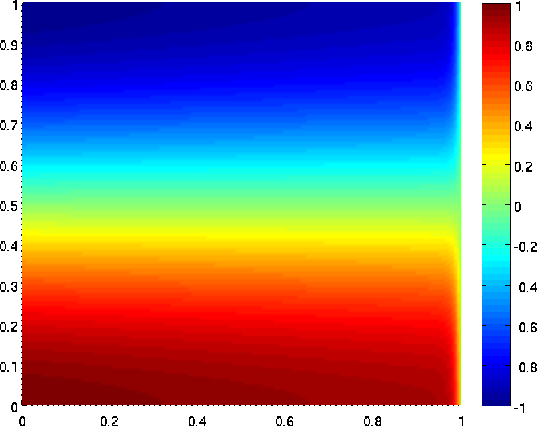
\includegraphics[scale=.37]{figs/wallBC_exact_u.png}
}
\subfigure{
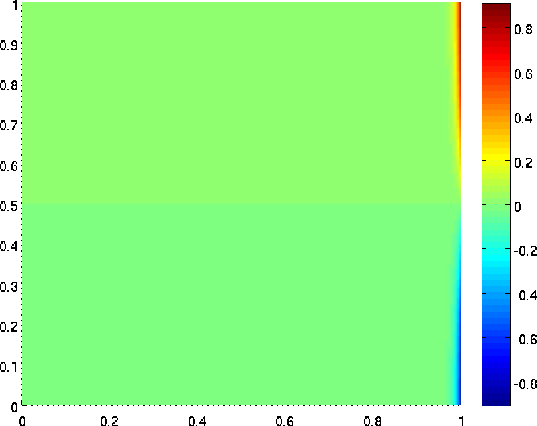
\includegraphics[scale=.37]{figs/wallBC_exact_sigx.png}
}
\subfigure{
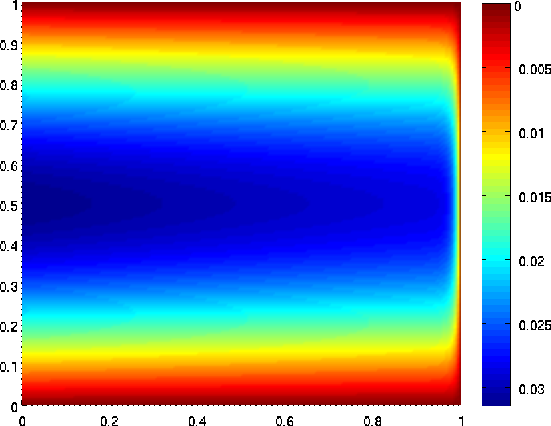
\includegraphics[scale=.37]{figs/wallBC_exact_sigy.png}
}
\caption{Solution for $u$, $\sigma_x$, and $\sigma_y$ for $\epsilon = .01$, $C_1 = 1$, $C_n=0$, $n\neq 1$}
\end{figure}

In each case, we begin with a square 4 by 4 mesh of quadrilateral elements with order $p=3$.  We choose $\Delta p = 5$, though we note that the behavior of DPG is nearly identical for any $\Delta p > 3$.  $h$-refinements are executed using a greedy refinement algorithm, where element energy error $e_K^2$ is computed for all elements $K$, and elements such that $e_K^2 \leq \alpha \max_K e_K^2$ are refined.  We make the arbitrary choice of taking $\alpha = .2$ for each of these experiments.  

\begin{figure}[h]
\centering
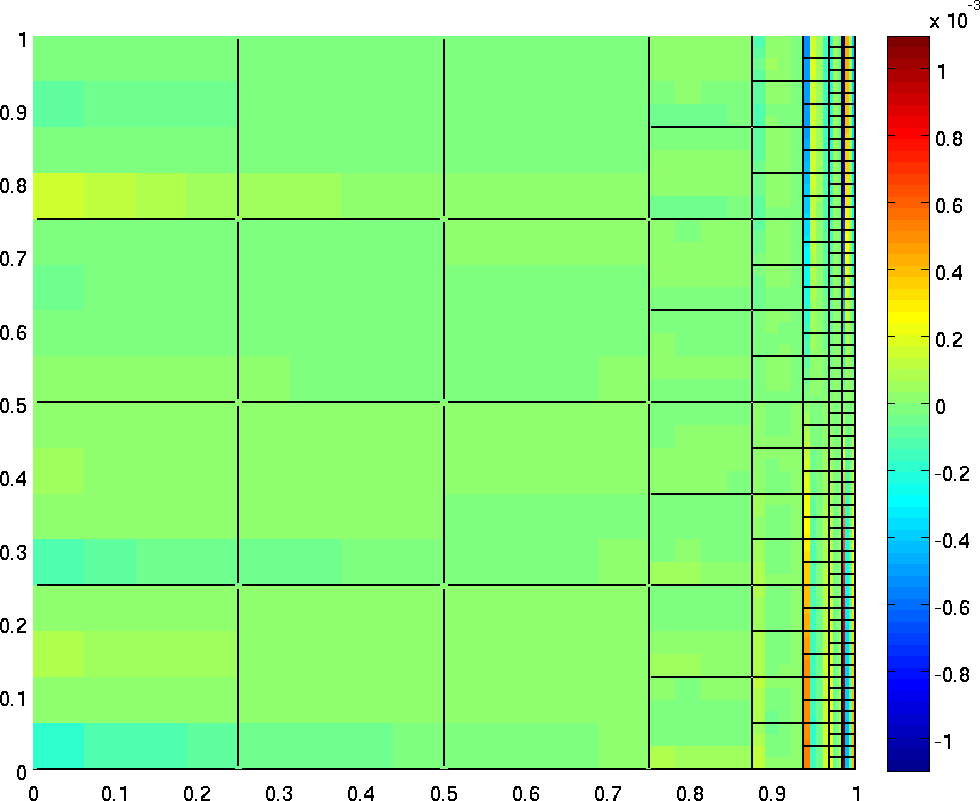
\includegraphics[scale=.4]{figs/u_pointdiff_wallBC.png}
\caption{Adapted mesh and pointwise error for $\epsilon=.01$}
\end{figure}

We are especially interested in the ratio of energy error and $L^2$ error.  Stability estimates imply that, using the above test norm, $\|u-u_h\|_{L^2} / \|u-u_h\|_E \sim C$ independent of $\epsilon$.  Figure~\ref{ratios_simple} seems to imply that, at least for this model problem, $C=O(1)$.  

\begin{figure}[h!]
\centering
\subfigure{
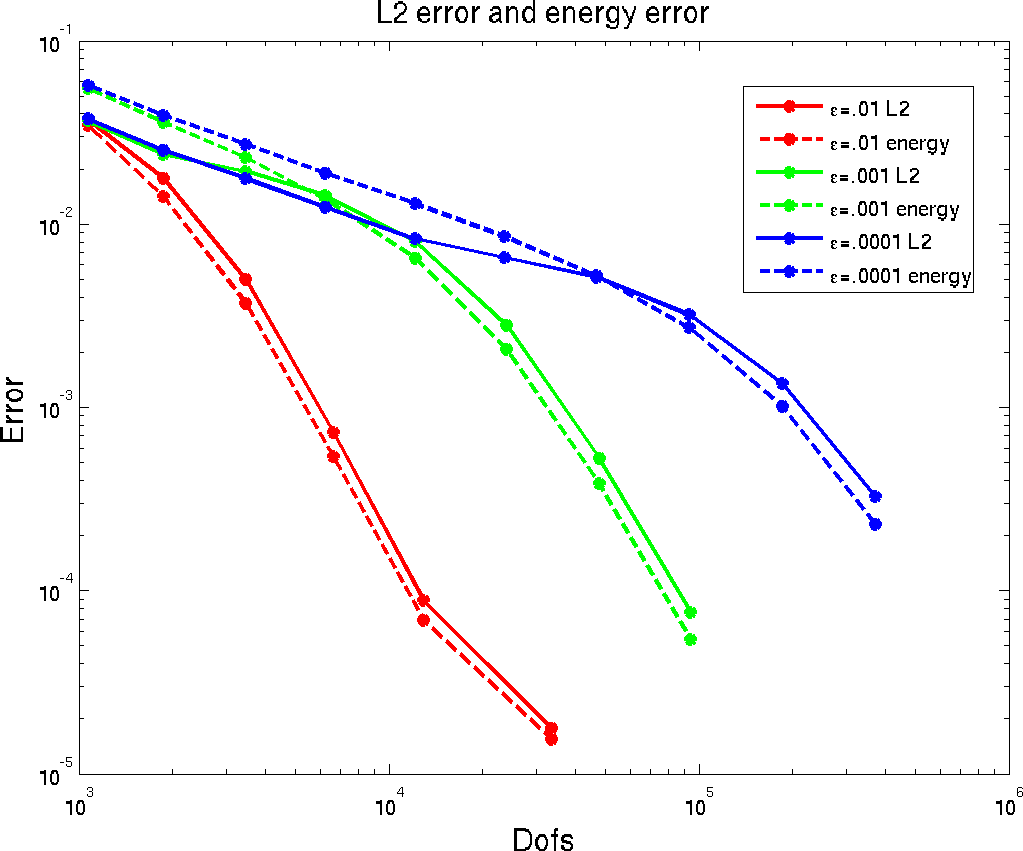
\includegraphics[scale=.38]{figs/errorrates_wallBC.png}
}
\subfigure{
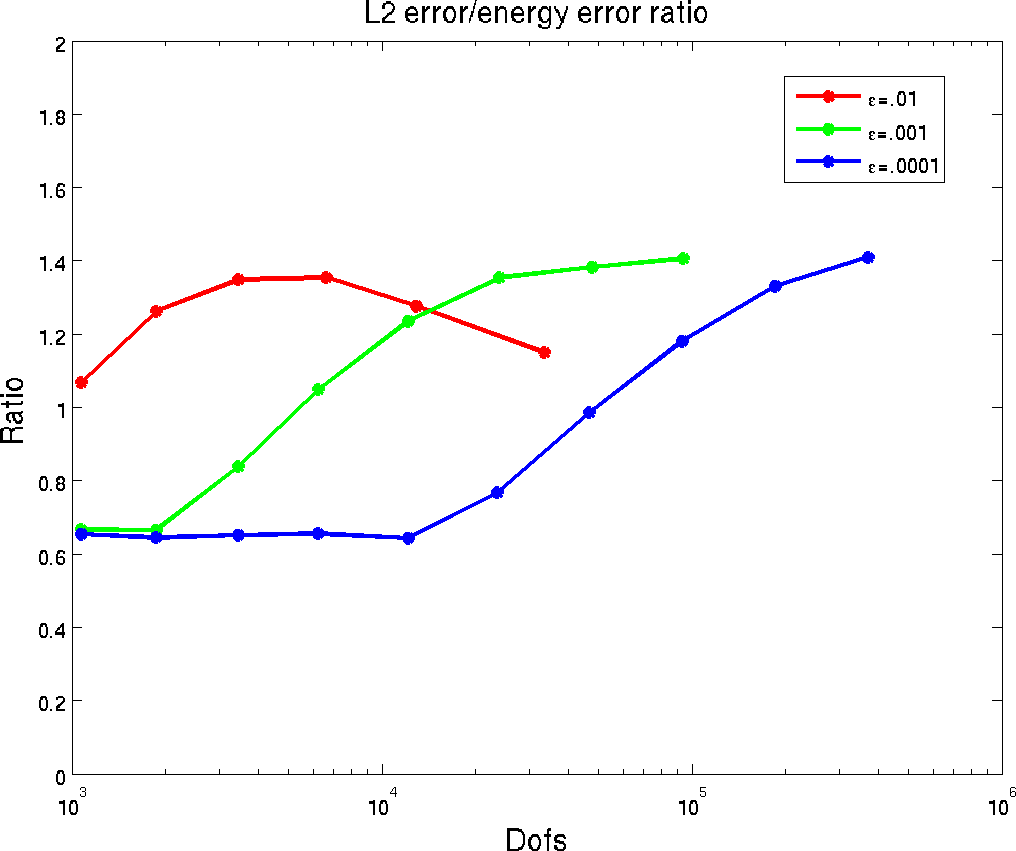
\includegraphics[scale=.38]{figs/L2energyratio_wallBC.png}
}
\caption{$L^2$ and energy errors, and their ratio for $\epsilon=.01$, $\epsilon=.001$, $\epsilon=.0001$}
\label{ratios_simple}
\end{figure}

The effect of the test norm on mesh dependence can be seen in the ratios of $L^2$ to energy error; as the mesh is refined, the constants in front of the $L^2$ terms for $v$ and $\tau$ converge to stationary values, and the ratio of $L^2$ to energy error transitions from a smaller to a larger value.  The transition point happens later for smaller $\epsilon$, which we expect, since the transition of the ratio corresponds to the introduction of elements of order $\epsilon$ through mesh refinement.  

\subsection{Neglecting $\sigma_n$} 

In practice, we will not have prior knowledge of $\sigma_n$ at the inflow, and will have to set $\beta_n u - \sigma_n = u_0$, ignoring the viscous contribution to the boundary condition.  The hope is that for small $\epsilon$, this omission will be negligible. Figure~\ref{ratios_noSigma} indicates that, between $\epsilon = .005$ and $\epsilon = .001$, the omission of $\sigma_n$ in the boundary condition becomes negligible, and both our error rates and ratios of $L^2$ to energy error become identical to the case where $\sigma_n$ is explicitly accounted for, well within the range of $\epsilon$ of physical interest. However, even for large $\epsilon = .01$, the $L^2$ error stagnates around $1e-3$, which is only $7%$ relative error. 

\begin{figure}[h!]
\centering
\subfigure{
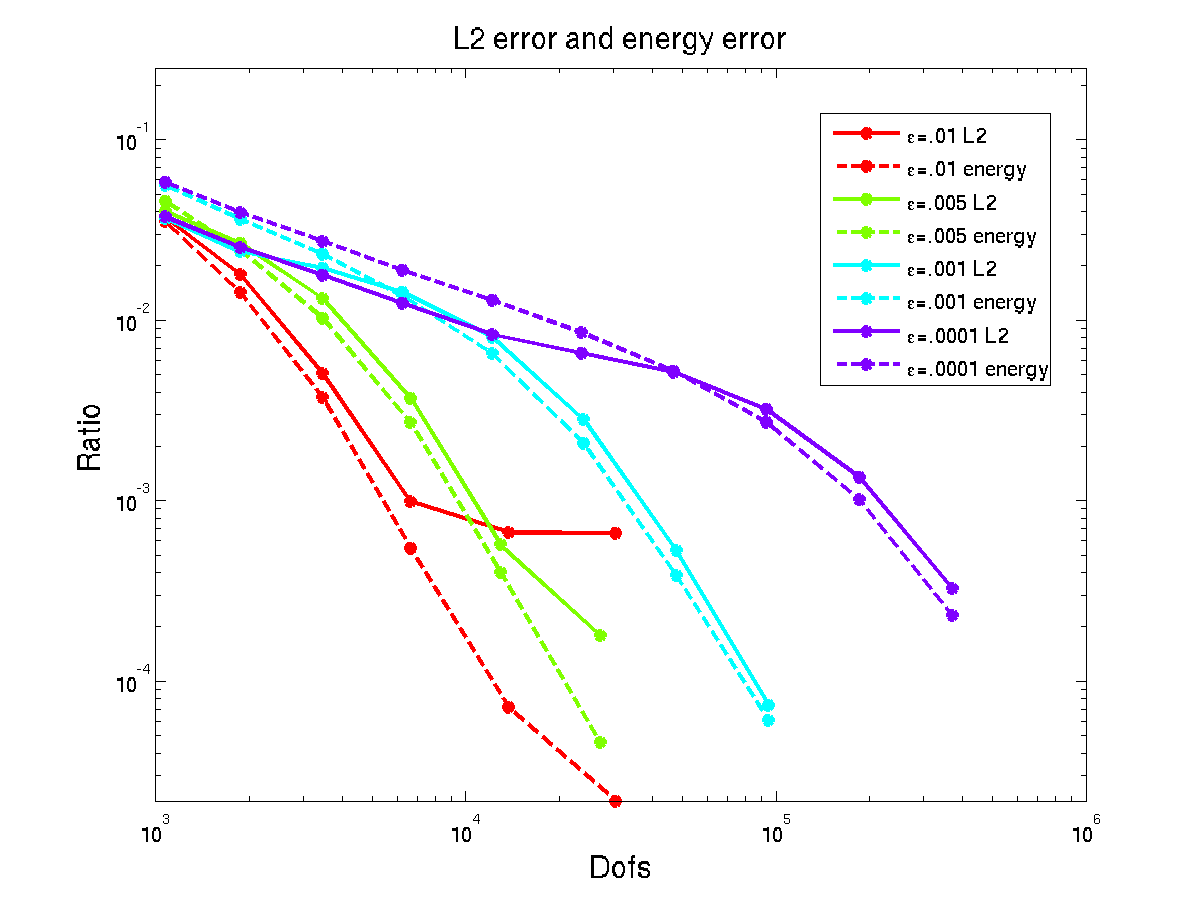
\includegraphics[scale=.38]{figs/rates_noSigma.png}
}
\subfigure{
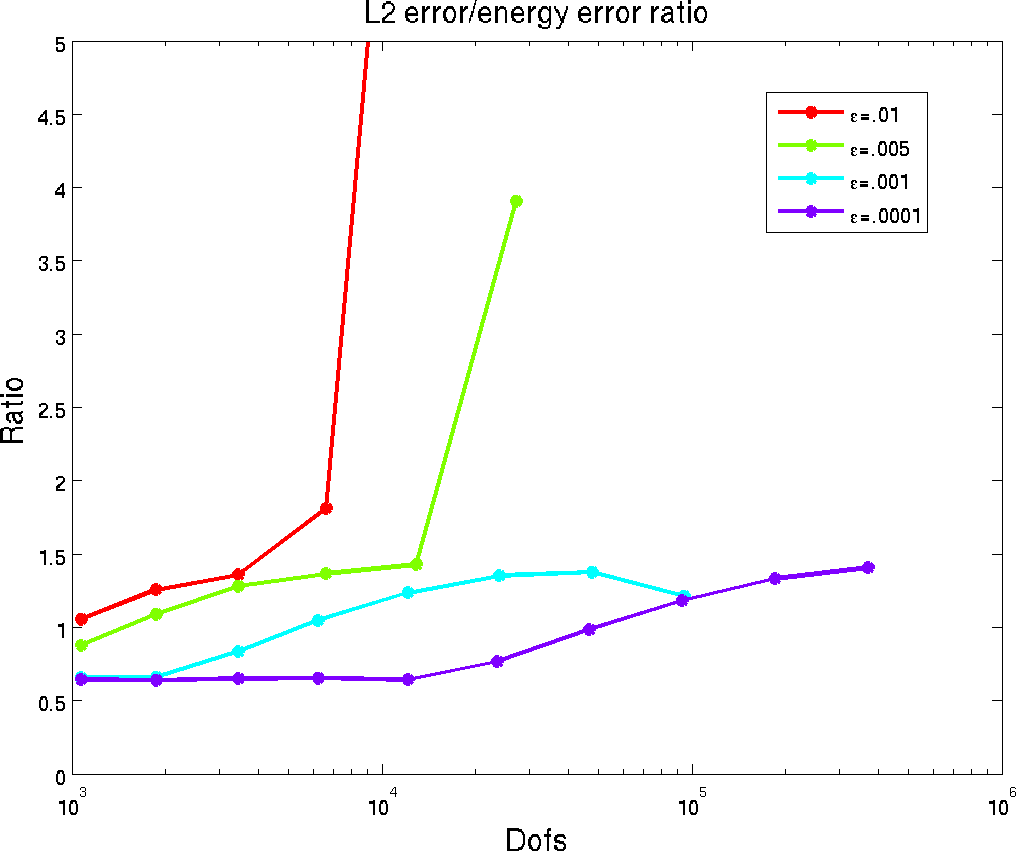
\includegraphics[scale=.38]{figs/ratio_noSigma.png}
}
\caption{$L^2$ and energy errors, and their ratio for $\epsilon=.01$, $\epsilon=.005$, $\epsilon=.001$, $\epsilon=.0001$}
\label{ratios_noSigma}
\end{figure}

\subsection{Discontinuous inflow data}

We note also that an additional advantage of selecting this new boundary condition is a relaxation of regularity requirements; as $\widehat{f}_n \in H^{-1/2}(\Omega)$, strictly discontinuous inflow boundary conditions are no longer ``variational crimes".  We use the discontinuous inflow data
\[
u_0(y) = \begin{cases}
(y-1)^2&, \quad y>.5\\
y^2&, \quad y\leq .5 
\end{cases}
\]


\section{Conclusions}
\bibliographystyle{plain}
\bibliography{paper}

\end{document}